\documentclass{article}

\usepackage[ruled,vlined]{algorithm2e}
\usepackage{graphicx}
\usepackage[margin=1.25in]{geometry}
\usepackage{fancyhdr}
\usepackage[utf8]{inputenc}
\usepackage{amsmath, amssymb}

%beginning of report
\begin{document}
\begin{titlepage}
\begin{figure}[!h]
    \centerline{
\includegraphics[scale=0.4]{Logo.png}}
    \centering
	\vspace{1cm}
    {\huge\bfseries RAMASSAGE DE DECHETS \\}
    {\huge\bfseries Projet algorithmique des graphes \\}
	\vspace{2cm}
	{\Large\itshape Benjamin DAYRES \\ Mohamed Taha SANDI \\ Samuel LANDEAU \\ Thomas COUTAYE \\}
	\vspace{1cm}
	{\large Encadr\'e par M.LAPOIRE\par}
    

\end{figure}
\end{titlepage}


\section{Introduction }
\subsection{Présentation du projet}
\hspace{0,5cm}  Le projet \`a  r\'ealiser consiste \`a concevoir et programmer des algorithmes de ramassage pour un robot charg\'e de collecter K d\'echets r\'epartis al\'etoirement
sur une grille carr\'ee de c\^ot\'e N. Le robot en question poss\`ede une vitesse de d\'eplacement constante unitaire et peut changer de direction en tournant sur lui m\^eme, avec un temps de changement
de direction d\'ependant de l'angle de rotation. Apr\`es avoir ramass\'e tous les d\'echets, le robot devra retourner \`a sa position initiale.
Le monde pourra \'eventuellement contenir des obstacles ayant une forme rectangulaire. Dans ce cas l\`a, le robot n'aura pas la possibilit\'e de les traverser et devra chercher un chemin alternatif
sans obstacles pour atteindre sa destination.

\subsection{ Objectif du projet}
\hspace{0,5cm} Le but du projet est de r\'epondre aux trois questions suivantes : \\
\hspace{1 cm} 
\begin{itemize}
\item Comment pourra-t-on mod\'eliser algorithmiquement les deux mondes o\`u \'evoluera notre robot ?
\item Quel algorithme nous permettra de resoudre de mani\`ere optimale notre probl\`eme, en fonction du nombre de déchet ?
\item Si jamais il devient impossible de calculer le chemin optimal, existe t'il tout de même un moyen d'en trouver des convenables ?
\end{itemize}

\section{ Mod\'elisation des deux mondes}
\hspace{0,5 cm}  Pour mod\'eliser le monde sans obstacles, on utilisera un graphe complet dont le nombre de sommets est \'egal aux nombre de d\'echets pr\'esents sur la grille plus notre 
position initiale. Ajoutons \`a cela que chaque ar\^ete de notre graphe portera un poids qui n'est autre que la distance euclidienne entre ses deux extremit\'es.

\begin{figure}[!h]
    \centerline{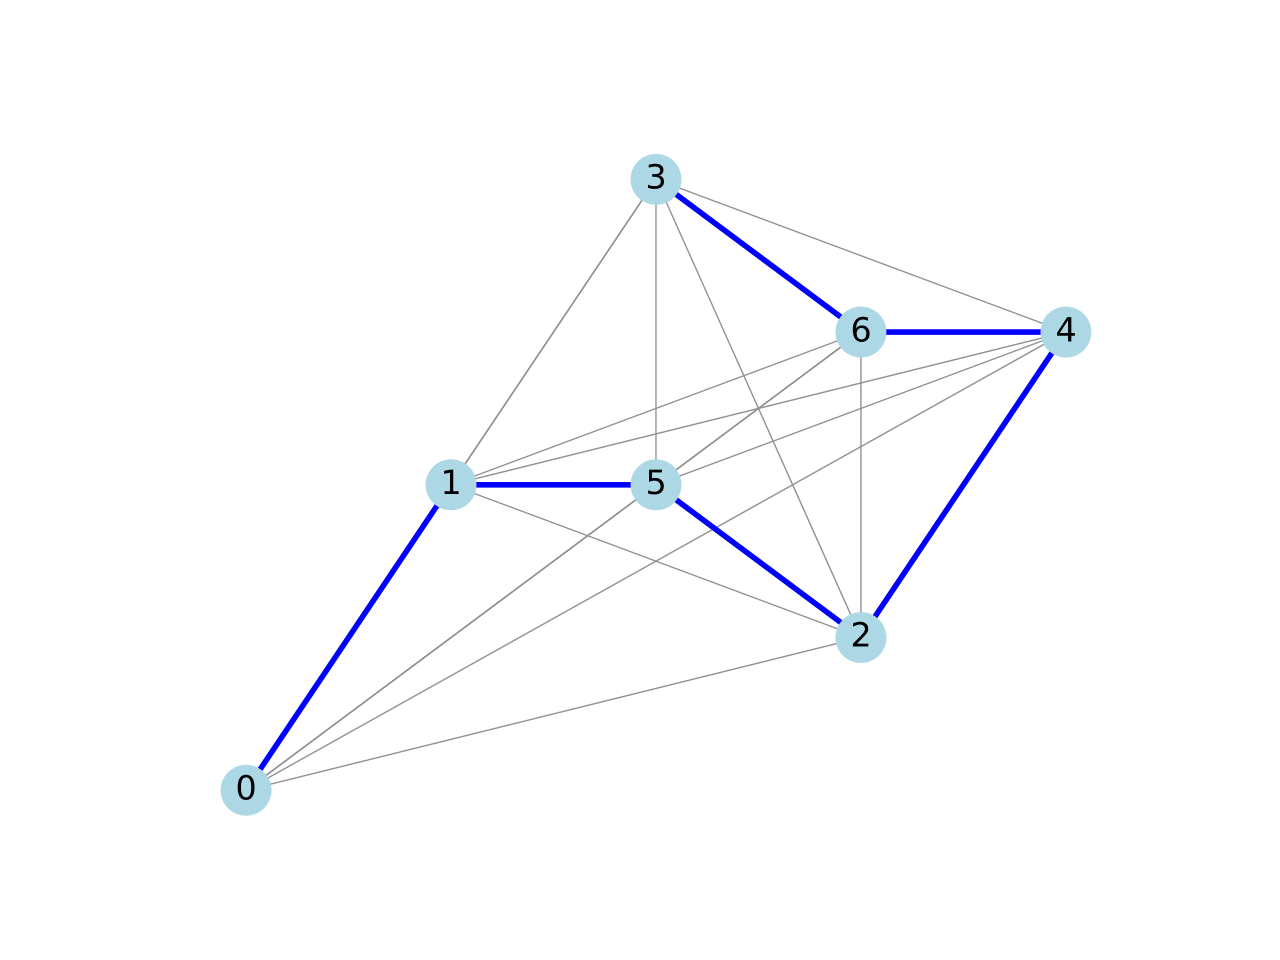
\includegraphics[scale=1]{best_path_arbitrary-1.png}}
    \caption{Exemple de graphe repr\'esentant un monde} 
  \end{figure}

Pour faire la distinction entre les monde avec et sans obstacles, nous collectons d'abord la liste des obstacles dans le monde avec obstacles. Puis pour chaque arêtes dans le graphe,
on v\'erifie si celle-ci traverse un obstacle. Si c'est le cas, nous donnons un poids infini à celle ci et nous stockons dans un tableau cette arête.

Ce tableau est ensuite parcourus, et pour chaque arête (u, v) de celui-ci, nous calculons le plus cours chemin allant de u à v, en incluant la possibilité de passer par les coins des rectangles obstacles. La longueur des chemin calculé devient alors le poids de (u, v).

Une fois le calcul fait, la présence d'obstacle n'a alors plus d'impact sur la complexité et la validité des algorithme de nous allons présenter.

\section{Nos algorithmes solutions}

Afin de résoudre ce problème de manière optimale, nous nous sommes posé la question suivante : comment trouver le chemin de ramassage optimal ?

Une solution évidente est de calculer tous les chemins possibles et de choisir le plus court. Si les $n$ déchets sont représentés par une suite sans répétition de nombre entre 1 et $n - 1$ et la position de départ par le sommet 0, on peut conclure qu'il faut calculer la longueur du chemin parcouru pour toute permutation de l'ensemble $[1 ; n]$.
Par exemple, si nous avons trois d\'echets 1, 2 et 3, nous pourrions \'enum\'erer toutes les six permutations possibles (123, 132, 213, 231, 312, 321) et calculer le co\^ut de chaque permutation pourt trouver la permutation avec le co\^ut minimum

Ainsi nous définissons les fonctions auxiliaires suivantes : \\

\begin{algorithm}
  \SetAlgoLined
  \KwResult{Un tableau contenant toutes les permutations de [1 ; n]}
  \caption{allPermutations(n)}
\end{algorithm}

\begin{algorithm}
    \SetAlgoLined
    \KwResult{Le temps que le robot prendra pour parcourir la permutation}
    time = 0\;
    currentVector = [0;1]\;
    \For{i from 0 to longueur(permutation) - 1}{
        time = time + poid(i, i+1)\;
        newVector = [pos[i][0] - pos[i+1][0] ; pos[i][1] - pos[i+1][1]]\;
        time = C * angle(currentVector, newVector)\;
        currentVector = newVector\;
    }
    return time\;
    \caption{permLength()}
  \end{algorithm}

  \begin{algorithm}[H]
    \SetAlgoLined
    \KwResult{Le meilleur chemin pour rammasser les déchets}
    permutations = allPermutations(n)\;
    bestPath = []\;
    minLength = $\infty$ \;
    \For{i from 0 to longueur(permutations)}
    {
        \If{permLength(permutations[i]) $<$ minLength}
        {
            minLength = permLength(permutations[i])\;
            bestPath = permutations[i]\;
        }
    }
    return bestPath\;
    \caption{bruteForce()}
  \end{algorithm}

  Cependant, on constate rapidement que cette approche a ses limites. En effet, le nombre de permutation pour un ensemble de taille $n$ est $!n$. La complexité en temps et en mémoire de notre algorithme est donc de $O(n!)$.
Par exemple, pour 10 d\'echets, il y a plus de 3,6 millions permutations possibles. Ainsi, l'algorithme force brute reste inefficace pour les instances de grande taille. \\

Bien qu'il soit possible de réduire la complexité en espace en fonction de l'implémentation selon un langage donné, en utilisant par exemple un itérateur en Python. La complexité en temps, elle, restera inchangée.\newline

Afin de trouver un autre algorithme, nous nous sommes demandés s'il n'existait pas déjà un problème documenté auquel nous pourrions ramener le nôtre.
Et, en effet, il est possible de ramener ce problème du ramassage de déchets au problème connu du voyageur de commerce.
Il existe de nombreux algorithmes permettant de résoudre ce problème, et nous nous sommes intéressés à l'algorithme de Christofides.

L'algorithme de Christofides donne une approximation de la solution du marchand de commerce.
Nous avons donc décidé d'utiliser une variante de celui-ci. En effet, l'algorithme de Christofides consiste à chercher l'arbre couvrant de poid minimum d'un graphe, puis d'effectuer un traitement sur celui-ci.
Cependant, nous allons simplement effectuer un parcours en profondeur du graphe, et ajouter les sommets dans l'ordre de ce parcours.
Pour calculer l'arbre couvrant de poids minimal, nous utiliserons l'algorithme de Kruskal.\newline

Nous supposerons connus ici une fonction \texttt{arbreMin(G)} qui applique l'algorithme de Kruskal sur G et une autre fonction \texttt{parcours(T)} qui effectue un parcours en profondeur de l'arbre T et ajoute les sommets en ordre suffixe dans une liste.\newline

  Ainsi, notre algorithme de résolution du problème de marchand de commerce est le suivante : 

  \begin{algorithm}
    \SetAlgoLined
    \KwResult{Tournée optimisé du TSP pour le graphe G}
    T = arbreMin(G)\;
    return parcours(T)\;
    \caption{tsp\_mst(G)}
  \end{algorithm}

%% Donner l'algo. Normalement il n'est pas nécessaire de décrire les algos de calcul de l'arbre couvrant minimal (Prim ou Kruskal) et de parcours en profondeur, car ils sont détaillé dans le cours.

  La solution obtenue par cette méthode n'est pas très satisfaisante et il est possible de très simplement améliorer ce résultat. \\ 

  En effet il existe une optimisation possible pour le problème du marchand de commerce, l'algorithme 2-optimisation.

  Cet algorithme consiste à chercher avec une heuristique une solution initiale de chemin le plus court, puis pour tout couple d'arêtes qui se croisent de vérifier le poid du chemin. Si décroiser les arêtes forme un meilleur chemin on continue.

  Cet algorithme se comporte en $\theta (n^2)$ sur la plupart des graphes et donc est plus rapide que l'algorithme "brute force", mais il n'assure absolument pas d'obtenir le chemin optimal, seulement une approximation minimale de ce chemin.\\
  \newline
  \begin{algorithm}[H]
    \SetAlgoLined
    \KwResult{Algo optimisé pour recherche de chemin}
    n = len(solution)\;
    amelioration = True\;
    \While{amelioration == True}{
       meilleur\_gain = 0\;
       amelioration = False\;
       \For{i in range(1,n-2)}{
          \For{j in range (i+1,n-1)}{
            gain = G[solution[i-1]][solution[j]]["weight"] + G[solution[i]][solution[j+1]]["weight"] - G[solution[i-1]][solution[i]]["weight"] - G[solution[j]][solution[j+1]]["weight"]\;
            \If{if gain < meilleur\_gain}{       
              \# Inversion des sous-tournées entre i et j
              solution[i:j+1] = reversed(solution[i:j+1])\;
              meilleur\_gain = gain\;
              amelioration = True\;
            }
          }
       }
    }
    return solution\;
    \caption{tsp\_2opt(solution,G)}
  \end{algorithm}

  Ainsi, en combinant les deux algorithme ci-dessus, il est possible de résoudre notre problème du robot ramasseur de déchets de manière satisfaisante même pour un grand nombre de points avec une complexité acceptable de $O(n^2)$

\section {Test et résultats}

Après avoir implémentés nos algorithmes, nous avons pu les tester afin de voir les différences entre eux, ainsi que les effets que les variations de
paramètres pouvait avoir sur les résultats. \\

Nous avons pu en premier lieu remarquer que la méthode brute force permettait d'avoir des résultats très concluant, notamment visible sur la figure
\ref{tsp_dechet}. Que ce soit avec obstacle ou non, les chemins calculés semblent parfaitement cohérent.
Malheureusement cette méthode est, comme nous l'avions prévu, très limitée lorsque le nombre de sommets à visiter augmente. Au delà de 10 sommets à
considérer, le temps pris par l'algorithme le rend déjà trop peu efficace pour continuer à l'utiliser. Cependant, l'algorithme 2-opt ne rencontre
aucunes difficultés à trouver des chemins pour des nombre de sommets bien plus grand, comme visible sur la figure \ref{2-opt_dechet}. \\

\begin{figure}[h!]
	\centering
	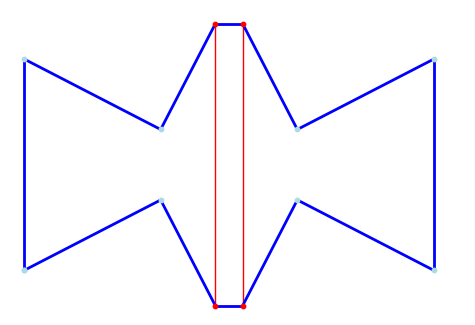
\includegraphics[scale=0.4]{image/Exemple8dechet.png}
	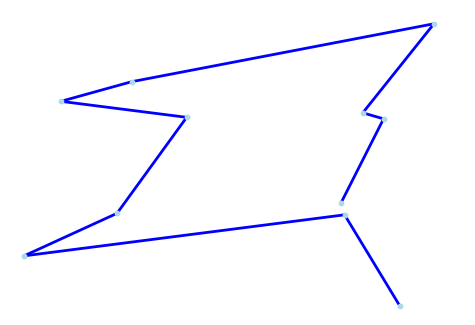
\includegraphics[scale=0.4]{image/Exmple10dechet.png}
	\caption{Recherche du chemin - Méthode Brute}
	\label{tsp_dechet}
\end{figure}

\begin{figure}[h!]
	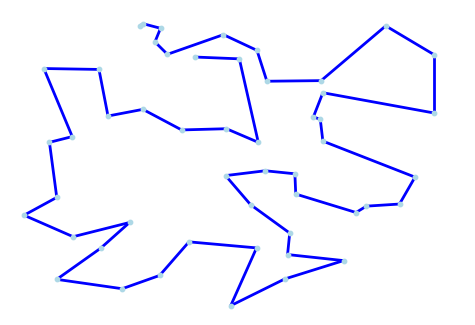
\includegraphics[scale=0.4]{image/Exmple50dechet.png}
	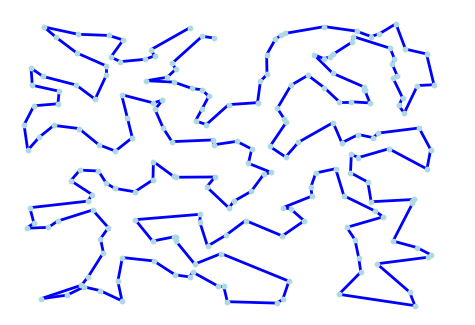
\includegraphics[scale=0.4]{image/Exemple200dechet.png}
	\caption{Recherche du chemin - Méthode 2-opt}
	\label{2-opt_dechet}
\end{figure}

Dans un second temps, nous avons voulu tester l'influence du temps de rotation sur les calculs du plus court chemin. Il est intéressant de voir à quel 
point le chemin s'en retrouve modifié lorsque l'on considère ou non un temps de rotation. Par exemple, sur les figures \ref{tsp_turn_1} et \ref{tsp_turn_2}, il est bien visible que le robot va se mettre à prioriser des trajectoires rectilignes ou presque afin de minimiser son temps de parcours, pouvant complètement modifier le parcours des sommets.

\begin{figure}[h!]
	\centering
	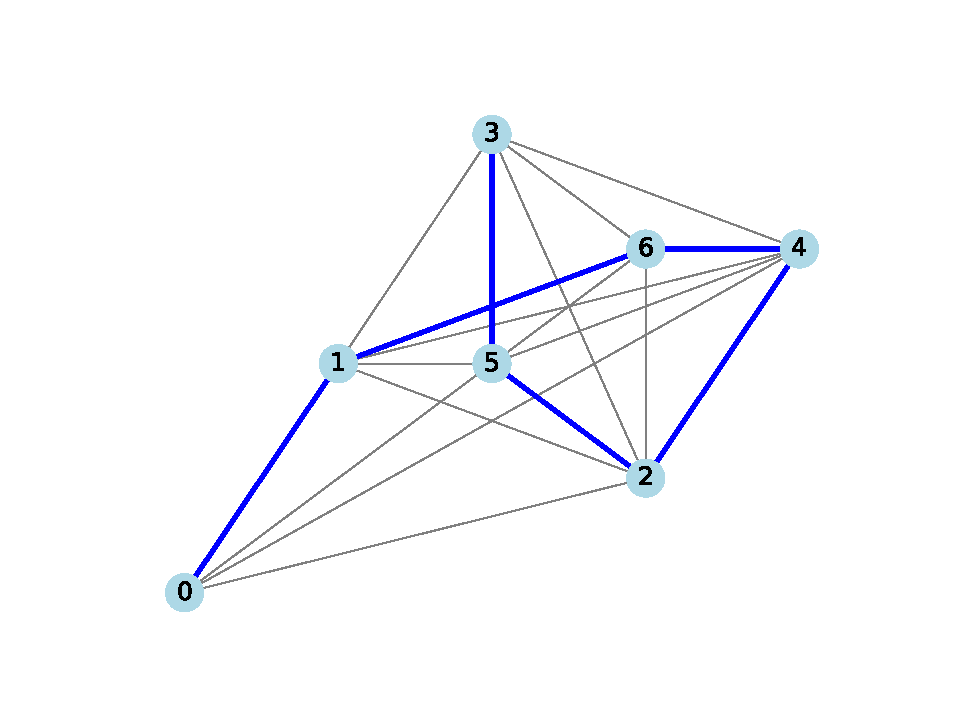
\includegraphics[scale=0.4]{figs/best_path_arbitrary_slow_turning.pdf}
	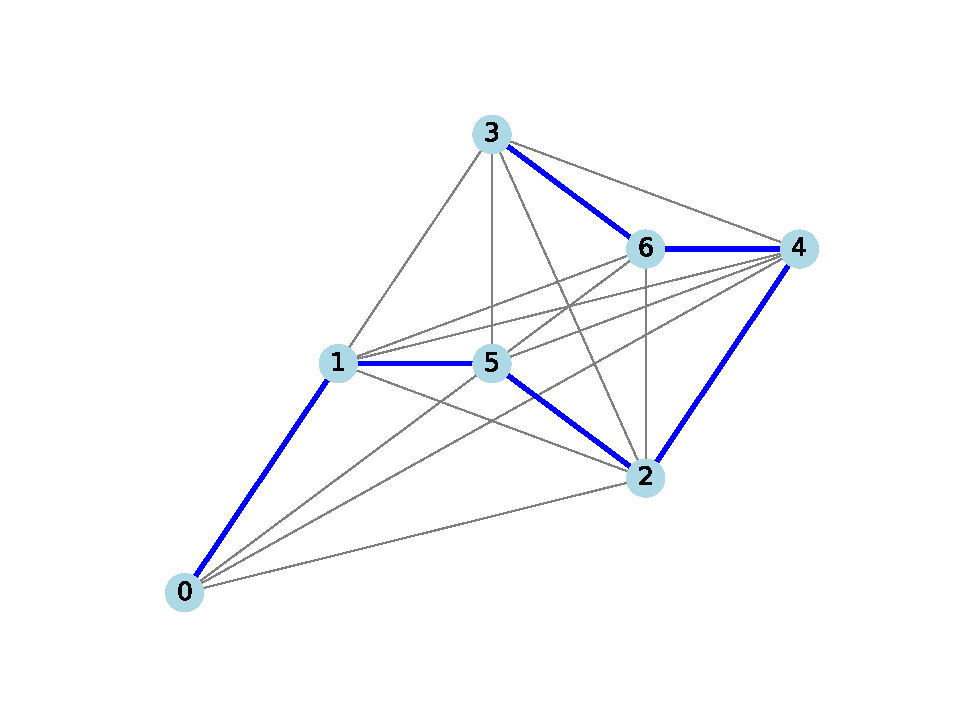
\includegraphics[scale=0.4]{figs/best_path_arbitrary.pdf}
	\caption{Recherche du chemin - Méthode Brute avec et sans rotation}
	\label{tsp_turn_1}
\end{figure}
\begin{figure}[h!]
	\centering
	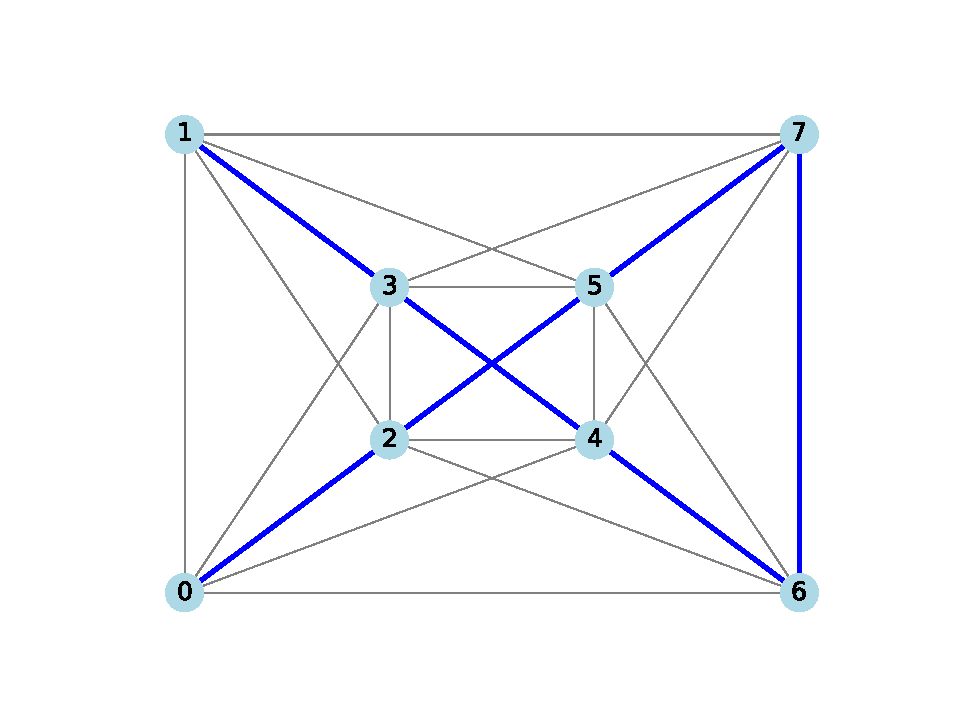
\includegraphics[scale=0.4]{figs/best_path_data1_slow_turning.pdf}
	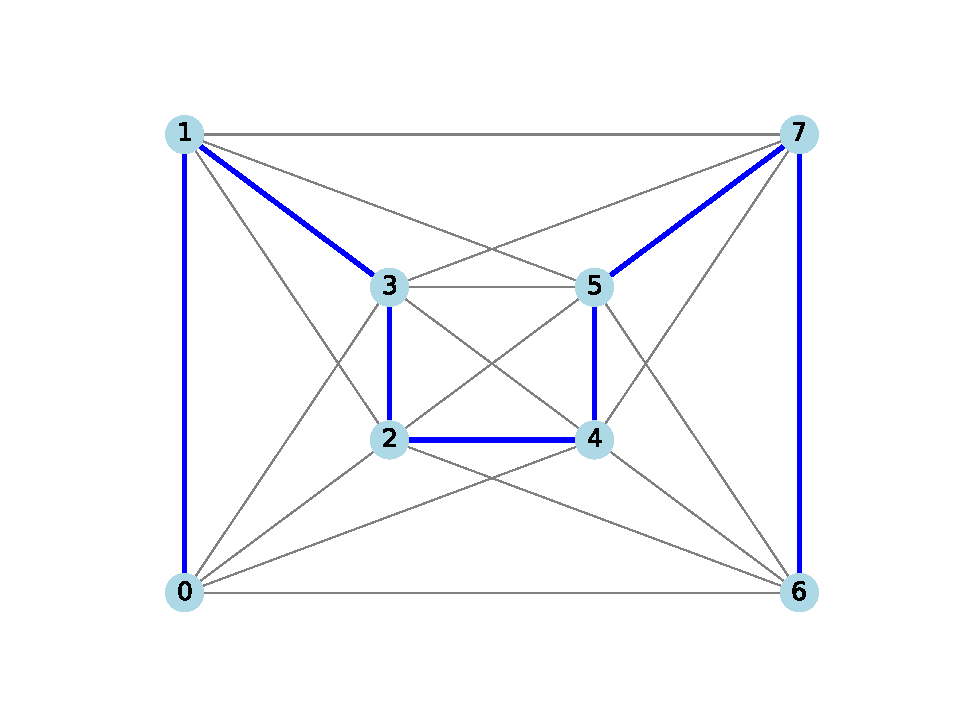
\includegraphics[scale=0.4]{figs/best_path_data1.pdf}
	\caption{Recherche du chemin - Méthode Brute avec et sans rotation}
	\label{tsp_turn_2}
\end{figure}

\section{Répartition des rôles}

Nous allons maintenant détailler et expliquer les parties sur lesquels chacun a travaillé.

\subsection{Algorithmes}
Benjamin Dayres

Lors de l'exposition du problème, j'ai rapidement remarqué une similitude avec un problème sur lequel j'avais déjà travaillé dans le cadre de mes études : le voyageur de commerce.
J'ai donc essayé d'utiliser mes connaissances pour transformer celui-ci afin qu'il colle au problème du ramassage de déchet. Les deux principales différences étaient les suivantes : la présence d'obstacle et le temps de rotation.
Les algorithmes utilisés ont donc été adapté afin de prendre ces deux contraintes en compte, et ainsi répondre, du mieux possible, au problème posé. \newline

Il est à noter un petit regret cependant, même si la gestion du temps de rotation fonctionne, 
elle n'est que très peu prise en compte dans le second algorithme présenté (Adaptation de Christofides) : seule la distance final est impacté par les variations de la valeur C, les chemins resteront les mêmes peu importe celle-ci. 
Cela peut s'expliquer par l'impossibilité de calculer à l'avance le temps que prendra le robot pour tourner si l'on ne connaît pas le chemin.

\subsection{Mod\'elisation des deux mondes}
Mohamed Taha SANDI

Apr\`es ma premi\`ere lecture du sujet, j'ai pens\'e que la repr\'esentation de notre monde se fera par une matrice d'adjascence de taille $N^2$ avec N la largeur du monde, mais je me suis 
vite aper\c{c} que cette approche n'\'etait pas valide vu qu'elle \'etait gourmande en terme de m\'emoire et prenait en consid\'eration des informations inutiles par rapport au probl\`eme pos\`e. En effet, tout le monde peut \^etre reconstruit
en connaissant seulement la position des d\'echets, de plus l'information la plus importante dans le cadre de notre projet est la distance euclidienne entre ces derniers vu qu'on travaille dans un espace euclidien 
de dimension deux. C'est pour ces raisons qu'on a d\'ecid\'e de repr\'esenter notre monde par une succession de coordonn\'ees repr\'esentant l'ensemble des d\'echets.


\subsection{Lecture des données}
Samuel LANDEAU

J'ai pour ma part principalement travaillé sur le fait d'apprendre comment traiter un fichier texte passé en paramètre pour le transformer en données
"lisibles" pour nos algorithmes, afin de pouvoir m'occuper de cette partie du projet. Il était important de bien communiquer avec les autres membres du 
projet pour transmettre les données dans le bon format (ne pas transmettre des listes à la place de tuples).

\subsection{Exemple et interprétation des données}

Pour moi, j'ai travaillé sur l'environnement de test avec des jeux de données que l'on a pu utilisé pour vérifier les algorithmes.
J'ai du prendre ou créer les jeux de données, les éditer et interpréter les résultats pour voir si les résultats étaient cohérent.



\end{document}
